\definecolor{rouge_inria}{RGB}{180,0,0}

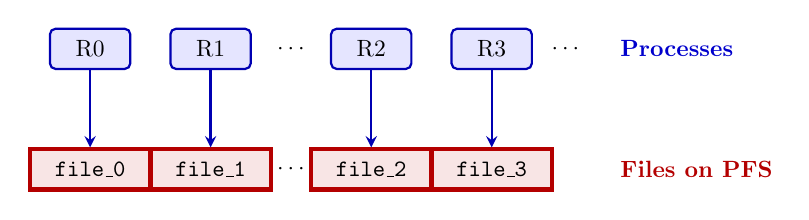
\begin{tikzpicture}[
    scale=0.85, every node/.style={transform shape},
    mpi/.style={rectangle, draw=blue!70!black, fill=blue!10, thick,
                minimum width=1.2cm, minimum height=0.6cm, rounded corners=2pt},
    pfs/.style={rectangle, draw=rouge_inria, fill=rouge_inria!10, ultra thick,
                minimum width=1.8cm, minimum height=0.6cm, align=center}
]
 
    % MPI Ranks
    \node[mpi] (m0) at (-3.8, 3) {R0};
    \node[mpi] (m1) at (-2.0, 3) {R1};
    \node      at   (-0.8,  3)   {$\cdots$};
    \node[mpi] (m2) at ( 0.4, 3) {R2};
    \node[mpi] (m3) at ( 2.2, 3) {R3};
    \node      at   ( 3.3,  3)   {$\cdots$};
    \node[anchor=west, text=blue!80!black, font=\bfseries] at (4.0, 3) {Processes};
 
    % Per-process files
    \node[pfs] (f0) at (-3.8, 1.2) {\texttt{file\_0}};
    \node[pfs] (f1) at (-2.0, 1.2) {\texttt{file\_1}};
    \node      at   (-0.8,  1.2)   {$\cdots$};
    \node[pfs] (f2) at ( 0.4, 1.2) {\texttt{file\_2}};
    \node[pfs] (f3) at ( 2.2, 1.2) {\texttt{file\_3}};
    \node[anchor=west, text=rouge_inria, font=\bfseries] at (4.0, 1.2)
        {Files on PFS};
 
    % Direct arrows Rank -> File (no coordination)
    \draw[->, >=stealth, thick, blue!70!black] (m0.south) -- (f0.north);
    \draw[->, >=stealth, thick, blue!70!black] (m1.south) -- (f1.north);
    \draw[->, >=stealth, thick, blue!70!black] (m2.south) -- (f2.north);
    \draw[->, >=stealth, thick, blue!70!black] (m3.south) -- (f3.north);
     
\end{tikzpicture}